\documentclass[12pt, a4paper, oneside]{report}

%% COMMANDS FOR THE TITLE PAGE CONTENT

% SW Author name (capitalized in its regular way)
\newcommand{\authorname}{Sean Allen Siegfreid R. Bugarin}

% SW Report Title (cannot exceed three lines)
% WORKING TITLE. The author chooses the final title.
\newcommand{\thetitle}{Evaluation-Guided Recovery in Agentic Retrieval-Augmented Generation: Diagnosing Failures and Verifying Repairs}

% Date of submission with normal capitalization.
% Use the format January 29, 2027.
% Fall 2026 final submission deadline per the Office of Signature Work guideline.
\newcommand{\submissiondate}{November 2, 2026}

% Mentor: First Name Last Name (normal capitalization)
\newcommand{\mentor}{Bing Luo}
% Mentor's Academic Unit (no abbreviations)
% Template default kept. Confirm this is the mentor's unit.
\newcommand{\mentoracademicunit}{Division of Natural and Applied Sciences}

% No co-mentor.
\newcommand{\comentor}{}

% Co-mentor's Academic Unit (no abbreviations)
% If the co-mentor is empty, the following will be ignored.
\newcommand{\comentoracademicunit}{}


%% PACKAGES

\usepackage[a4paper, margin=1in]{geometry}
\usepackage{parskip}

\usepackage{amsmath, amsthm}

% Office of Signature Work formatting: Times New Roman (or Garamond, Cambria,
% Arial) at 12 pt, double spaced, 1 inch margins. newtx supplies Times for
% text and math; amssymb is omitted because newtxmath provides its symbols.
\usepackage[T1]{fontenc}
\usepackage{newtxtext, newtxmath}
\renewcommand{\sfdefault}{\rmdefault}
\usepackage{graphicx}
\usepackage{xcolor}
\usepackage{longtable, booktabs, array}

\usepackage{upquote}
\usepackage{microtype}

\usepackage{titlesec}
\titleformat{\chapter}[display]
  {\sffamily\bfseries\huge}
  {\Large\chaptertitlename\ \thechapter}
  {2ex}
  {\titlerule\vspace{1ex}\filright\MakeUppercase}
  [\vspace{1ex}\titlerule]
\titleformat{\section}{\normalfont\sffamily\Large\bfseries}{\thesection}{1em}{}
\titleformat{\subsection}{\normalfont\sffamily\large\bfseries}{\thesubsection}{1em}{}
\titleformat{\subsubsection}{\normalfont\sffamily\normalsize\bfseries}{\thesubsubsection}{1em}{}

\usepackage[style=numeric-comp, url=false]{biblatex}
\addbibresource{references.bib}

% Orange text inside the \instructions command must not appear
% in the final version of your report. You can either delete it
% from your document, or redefine the command \instructions, by
% commenting out the definition here...
\newcommand{\instructions}[1]{}
\newcommand{\authornote}[1]{}

\newcommand{\code}[1]{\texttt{\detokenize{#1}}}

\usepackage{tikz}
\usetikzlibrary{arrows.meta, positioning}

\usepackage[allcolors=blue, colorlinks=true]{hyperref}
\usepackage{xurl}
\usepackage{bookmark}

\urlstyle{same}

\usepackage{calc}
\usepackage{xifthen}
\usepackage{etoolbox}

\usepackage{setspace}

\begin{document}

\thispagestyle{empty}

% About Majors at DKU
Background:  Duke Kunshan University (DKU) is an interdisciplinary institution that grants dual undergraduate degrees, an MOE Chinese degree and a degree from Duke University in Durham, United States. The principal structure of DKU majors is robustly interdisciplinary. No student confines their study to a single discipline (for example, biology or economics). Instead, all students engage in broad inquiry related to a subject or question (for example, political economy or global health) and take a wide variety of courses related to that area (for example, in public policy, history, ethics, or economics). As a result, our graduates are prepared to engage in a wide variety of inquiries using multiple methodologies to address complex issues that require interdisciplinary approaches.  

This has implications for our vision and expectations of undergraduate theses and design projects, which reflect this broad interdisciplinary training. At DKU, every student completes a two-year project known as signature work which consists of multiple interconnected parts including thematic courses, experiential learning, capstones, and a final product. It seeks to integrate students’ interdisciplinary educational experience and culminates in the creation of a product in a scholarly, creative, or applied nature in lieu of an undergraduate thesis or design required by JED. Because DKU encourages students to cultivate their independence and creativity as one of its institutional student learning outcomes, the student-led signature work projects often reflect students’ own particular interdisciplinary interests and training.  In addition, signature work has an intensive emphasis on problem-solving and skill-development which is much needed for any interdisciplinary inquiry; thus, students’ final products are evidence of transferrable skills that students have acquired and demonstrated through the 2-year program, rather than content knowledge narrowly defined by disciplinary training. 
 
In sum, while the Chinese major declared with any given student might be construed narrowly, the experience of our students is much broader—and intentionally so.  This is a distinctive feature of our curriculum, and this distinctiveness results in broadly interdisciplinary submissions from our graduates’ submitting theses or design projects. We have designed this to prepare our students for a wide variety of graduate programs in China and the West, where interdisciplinary training is a competitive advantage.

%%%%%%%%%%%%%%%%%%%%%%%%%%%%%%%%%%%%%%%%%%%%%%%%%%%%%%%%%%%%%%%%

%% DO NOT CHANGE DIRECTLY THE CONTENTS OF THE TITLE PAGE.
%% TO CUSTOMIZE THE TITLE PAGE CHANGE THE DEFINITIONS OF THE COMMANDS
%% \authorname, \thetitle, \submissiondate
%% \mentor, \mentoracademicunit
%% \comentor, \comentoracademicunit

\begin{titlepage}

\vspace*{\bigskipamount}

\begin{center}
{\sffamily\LARGE\bfseries\MakeUppercase\thetitle\par}

\bigskip

by

\bigskip

{\Large \authorname}

\bigskip

Signature Work Product, in partial fulfillment of the \\
Duke Kunshan University Undergraduate Degree Program

\bigskip

\emph{\submissiondate}

\bigskip

Signature Work Program \\
Duke Kunshan University

\end{center}

\vfill

\textbf{\textsf{APPROVALS}}

\vspace{3em}\hrule\par
Mentor: \mentor, \mentoracademicunit

\ifthenelse{\equal{\comentor}{}}{}{
\vspace{3em}\hrule\par
Co-Mentor: \comentor, \comentoracademicunit
}

\end{titlepage}

%%%%%%%%%%%%%%%%%%%%%%%%%%%%%%%%%%%%%%%%%%%%%%%%%%%%%%%%%%%%%%%%

% Front matter
\clearpage
\pagenumbering{roman}

%%%%%%%%%%%%%%%%%%%%%%%%%%%%%%%%%%%%%%%%%%%%%%%%%%%%%%%%%%%%%%%%

% Only top-level units (chapters) should appear in the TOC
\setcounter{tocdepth}{0} 
\tableofcontents

\doublespacing % τοῖς κείνων ρήμασι πειθόμενοι

%%%%%%%%%%%%%%%%%%%%%%%%%%%%%%%%%%%%%%%%%%%%%%%%%%%%%%%%%%%%%%%%

\chapter*{Abstract}
\addcontentsline{toc}{chapter}{Abstract}

% Abstract in English

This project asks whether runtime evaluation in an agentic RAG system can
identify why an answer failed, choose a corrective action, and correctly
judge whether that action improved the answer. A single-hop loop evaluates
each answer with a language-model judge and a span check, diagnoses a
failure, recovers by expanding retrieval or abstaining, and verifies the
result. It is compared with a retrieve-once baseline on three small
collections (88 questions). On answerable questions the contains-answer
count was unchanged on two collections and rose by one on the third.
Abstention on unanswerable questions rose by one on two collections. The
loop used about three times as many chat calls. Runtime verification
agreed with an offline gold check on 24 of 25 recovered runs, but 20 of
those 25 were labeled still failing, and 18 of those 20 were already
gold-accepted. A 40-item judge audit agreed with human labels on 39 calls
per flag and still accepted one wrong-source answer. The runs do not show
that evaluation-guided recovery reliably improves answers. They show that
the loop's self-assessment is easy to agree with when little changes, and
that the judge can over-trigger recovery and miss a source error.

\textbf{Keywords:} retrieval-augmented generation; agentic RAG; runtime
evaluation; failure recovery; recovery verification.

\vspace{4\bigskipamount}


%%%%%%%%%%%%%%%%%%%%%%%%%%%%%%%%%%%%%%%%%%%%%%%%%%%%%%%%%%%%%%%%

\chapter*{Acknowledgements}
\label{acknowledgements}
\addcontentsline{toc}{chapter}{Acknowledgements}

I thank Bing Luo for mentoring this Signature Work, and Mingxi, a doctoral
student in his group, who guided my research on ChatDKU. That work on
evaluating a campus question-answering system is what led to the question
this project studies.

\newpage

%%%%%%%%%%%%%%%%%%%%%%%%%%%%%%%%%%%%%%%%%%%%%%%%%%%%%%%%%%%%%%%%

% Add captions to your figures for them to appear in the List of Figures.
% Alternatively, comment out the next two lines if there are no tables 
% in your document.
\addcontentsline{toc}{chapter}{List of Figures}
\setcounter{tocdepth}{1}
\listoffigures\newpage

%%%%%%%%%%%%%%%%%%%%%%%%%%%%%%%%%%%%%%%%%%%%%%%%%%%%%%%%%%%%%%%%

% Add captions to your tables for them to appear in the List of Tables.
% Alternatively, comment out the next two lines if there are no tables 
% in your document.
\addcontentsline{toc}{chapter}{List of Tables}
\setcounter{tocdepth}{1}
\listoftables\newpage

%%%%%%%%%%%%%%%%%%%%%%%%%%%%%%%%%%%%%%%%%%%%%%%%%%%%%%%%%%%%%%%%

% Main matter
\clearpage
\pagenumbering{arabic}

%%%%%%%%%%%%%%%%%%%%%%%%%%%%%%%%%%%%%%%%%%%%%%%%%%%%%%%%%%%%%%%%

\chapter{Introduction}
\label{introduction}

\section{Motivation}

This project grew out of my work as a researcher on ChatDKU, a campus
question-answering assistant at Duke Kunshan University. Most of that role
was evaluation. A score told us how often the assistant was right. It did
not tell us what had gone wrong or which change would help: a low score
could come from retrieval, from the documents, or from the model's answer.
I also started an automated evaluation and did not finish it. That gap
between scoring a system and knowing how to repair it is the starting
point for this work.

\section{Problem and Research Question}

A retrieval-augmented generation (RAG) system retrieves passages and asks
a language model to answer from them~\cite{lewis2020rag}. Failures are
often silent: the wrong passage, a missing fact, or a fluent answer that
adds unsupported claims. An agentic RAG system does not stop after one
attempt. It evaluates, diagnoses, recovers (rewrite, retrieve more, or
abstain), and checks whether the correction helped:

\begin{center}
act $\rightarrow$ evaluate $\rightarrow$ diagnose $\rightarrow$ recover
$\rightarrow$ verify $\rightarrow$ accept, retry, or abstain.
\end{center}

The last step uses the same kind of automatic evaluation that detected the
failure. If that evaluator is wrong, the system can accept a worse answer
or claim a repair that did not happen.

\begin{quote}
Can runtime evaluation in an agentic RAG system identify why an answer
failed, choose a corrective action suited to that failure, and correctly
judge whether the correction improved the answer?
\end{quote}

The question is measured in three parts: (1)~how the evaluation-guided
loop compares with a retrieve-once baseline; (2)~how often the system's
verification verdict agrees with an offline gold check; (3)~how often the
judge agrees with a human reader. Retrieval is single-hop; that limit is
stated in Scope, not in the question.

\section{Background and Prior Work}

RAG pairs a retriever with a generator that conditions on what was
retrieved~\cite{lewis2020rag}. Surveys describe a move from that fixed
pipeline toward modular and agentic RAG, in which an agent decides when
and how to retrieve again~\cite{gao2023ragsurvey,singh2025agenticrag}.
Adaptive systems act on a runtime signal: FLARE retrieves when token
confidence is low~\cite{jiang2023flare}; Self-RAG trains reflection
tokens~\cite{asai2024selfrag}; CRAG scores retrieved documents and
refines or replaces them~\cite{yan2024crag}; Adaptive-RAG routes by
question complexity~\cite{jeong2024adaptiverag}. They report task
accuracy after the action. They do not measure whether the system's own
claim that the action helped was correct.

Offline tools diagnose after the run. RAGAs, ARES, and RAGChecker score
faithfulness, relevance, and module-level
errors~\cite{es2024ragas,saadfalcon2024ares,ru2024ragchecker}. Barnett
et al.\ list seven RAG failure points and note that validation is only
feasible during operation~\cite{barnett2024sevenfailure}. Joren et al.\
separate insufficient context from unused context and use sufficiency to
guide abstention~\cite{joren2025sufficient}. Language-model judges can
match human preference rates but show position and verbosity
biases~\cite{zheng2023judging,wang2024fair}. Self-correction works when
feedback is reliable and often fails without it
\cite{huang2024cannot,kamoi2024selfcorrection,shinn2023reflexion}.
Agent-failure taxonomies treat diagnosis and repair as separate
problems~\cite{cemri2025mast,zhu2025agentdebug}. Abstention is a standard
way to reduce hallucination~\cite{wen2025abstention}.

Those systems either act at runtime and report end-task accuracy, or
diagnose offline. This project does both: it diagnoses and recovers at
runtime, records the loop's verdict, and scores that verdict against gold
the running system never sees, and against a human check of the judge.
The contribution is a measurement of that self-assessment, not a new
retriever.

\section{Scope and Limits}

The work is limited in four deliberate ways.

\begin{itemize}
\item \textbf{Single-hop retrieval.} Each question retrieves once, then
  at most two recoveries that may retrieve again. Multi-hop chaining is
  out of scope.
\item \textbf{Small, controlled collections.} Two fictional sets and one
  set of public Duke Kunshan facts, written so each gold answer can be
  checked by hand.
\item \textbf{Runtime signals never read the answer key.} The judge,
  diagnosis, policy, and verifier see only the question, the passages,
  and the answer. Gold is used only offline.
\item \textbf{Software is the primary deliverable.} Experimental claims
  are limited to the recorded runs on these collections.
\end{itemize}

%%%%%%%%%%%%%%%%%%%%%%%%%%%%%%%%%%%%%%%%%%%%%%%%%%%%%%%%%%%%%%%%

\chapter{Material and Methods}
\label{material-and-methods}

\section{System, Models, and Collections}

The primary product is a working agentic RAG application. A FastAPI
server exposes the engine and serves a static web console. An operator
creates a system, uploads a document collection, asks a question, and
sees the retrieved passages, the generated answer, the judge flags, the
diagnosis, and any recovery the loop applied. The console can run
recoveries automatically or pause for confirmation. Every query writes
one JSON trace that is never overwritten: passages, flags, diagnosis,
each recovery attempt, and the verification outcome. A recovery applied
after confirmation is a child trace linked to its parent. The study
runs below used the same engine in automatic mode. Figure~\ref{fig:loop}
shows the loop.

\begin{figure}[htbp]
\centering
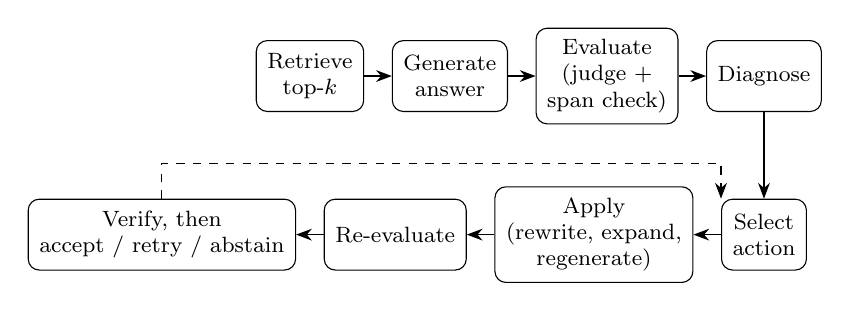
\begin{tikzpicture}[
  node distance=0.55cm and 0.35cm,
  box/.style={draw, rounded corners, align=center, font=\footnotesize\sffamily,
              minimum height=0.9cm, inner sep=4pt},
  arr/.style={-{Stealth[length=2mm]}}]
\node[box] (ret) {Retrieve\\top-$k$};
\node[box, right=of ret] (gen) {Generate\\answer};
\node[box, right=of gen] (judge) {Evaluate\\(judge +\\span check)};
\node[box, right=of judge] (diag) {Diagnose};
\node[box, below=1.1cm of diag] (sel) {Select\\action};
\node[box, left=of sel] (apply) {Apply\\(rewrite, expand,\\regenerate)};
\node[box, left=of apply] (rejudge) {Re-evaluate};
\node[box, left=of rejudge] (ver) {Verify, then\\accept / retry / abstain};
\draw[arr] (ret) -- (gen);
\draw[arr] (gen) -- (judge);
\draw[arr] (judge) -- (diag);
\draw[arr] (diag) -- (sel);
\draw[arr] (sel) -- (apply);
\draw[arr] (apply) -- (rejudge);
\draw[arr] (rejudge) -- (ver);
\draw[arr, dashed] (ver.north) -- ++(0,0.45) -| (sel.north west);
\end{tikzpicture}
\caption{One query through the evaluation-guided loop. The dashed arrow is
a retry while the recovery budget remains.}
\label{fig:loop}
\end{figure}

Generation, judging, and query rewriting use \code{gpt-4o-mini} at
temperature~0 with a JSON response. Passages are embedded with
\code{text-embedding-3-small}. The same chat model serves as generator and
judge. Documents are split into 500-character chunks with 80-character
overlap. A query returns the $k=4$ nearest chunks by cosine similarity.

Each collection is a folder of plain-text documents plus a gold question
set. A gold row records the question, whether it is answerable, accepted
answer strings, and supporting documents. Unanswerable questions are
included so that abstention can be scored. Table~\ref{tbl:corpora} lists
the three study collections. The fictional sets contain superseded
notices, near-duplicate facilities, and expected facts that the documents
never state. The author reviewed every gold row on 11 October 2026; no
row changed.

\begin{table}[htbp]
\centering
\footnotesize
\setlength{\tabcolsep}{5pt}
\begin{tabular}{@{}lllrrr@{}}
\toprule
Collection & Domain & Source & Files & Answerable & Not answerable \\
\midrule
Harbor Institute & Research campus & Fictional & 11 & 22 & 10 \\
Duke Kunshan University & University campus & Public facts & 14 & 30 & 10 \\
Kestrel Aero Components & Aerospace parts & Fictional & 16 & 12 & 4 \\
\bottomrule
\end{tabular}
\caption{Study collections and gold question counts.}
\label{tbl:corpora}
\end{table}

\section{Evaluation, Recovery, and Verification}

A grounding judge reads the question, the retrieved chunks, and the
answer, and returns two flags: whether the evidence could answer the
question, and whether every fact in the answer is stated in the evidence.
It is forbidden to use outside knowledge; fluency is not support; it never
sees gold. A span check then extracts clock times, emails, ordinals,
specification tokens, and numbers of three or more digits, and rejects an
answer if any of them is absent from the retrieved text. A retrieval
signal, computed from similarity scores only, marks a hit as weak when
the top score is below $0.15$ or the relative margin
$(s_1-s_2)/s_1$ is below $0.02$. Those thresholds were set by hand.

On the first pass, an unsupported answer with sufficient evidence is
\emph{unsupported generation}. Insufficient evidence is classified only
after a second retrieval: if evidence becomes sufficient, a
\emph{retrieval miss}; if not, \emph{evidence insufficiency}.
Table~\ref{tbl:actions} is the default policy. The study budget is two
recoveries. A later action never repeats an earlier one. A last expand or
regenerate that still fails the span check, or that still lacks evidence,
becomes an abstention. Abstaining does not count against the budget.

\begin{table}[htbp]
\centering
\small
\begin{tabular}{@{}p{4.4cm}p{2.2cm}p{7.2cm}@{}}
\toprule
State & Action & Effect \\
\midrule
Unsupported generation & Regenerate & New answer from the same chunks. \\
Evidence insufficient (first pass) & Rewrite & New query; answer again only
if the new evidence is sufficient. \\
Judge accepts, retrieval signal weak & Expand & Same query, $k=4$ to $12$
(cap 20). \\
Evidence insufficient after rewrite & Abstain & ``I do not know based on
the retrieved documents.'' \\
No failure & Accept & Answer kept. \\
\bottomrule
\end{tabular}
\caption{Default recovery policy.}
\label{tbl:actions}
\end{table}

A rewrite or regenerate that still fails escalates to expand. After a
failed rewrite, a first-pass answer the judge called supported is kept.
The web console can apply recoveries automatically or wait for an
operator; the study runs used automatic mode.

The verifier compares flags before and after recovery:
\emph{improved} (a flag false to true), \emph{degraded} (true to false),
\emph{still failing} (evidence or answer still failing), or
\emph{unchanged}. An abstention is never improved while evidence is
insufficient or a rejected fact remains. Offline scoring, which the
running system never sees, reports contains-answer and token F1 on
answerable questions, abstention on unanswerable and answerable questions,
and retrieval hit rate. Results are reported per collection, not as one
pooled score.

\section{Study Runs and Human Review}

Each collection's full gold set is run once as a retrieve-once
\emph{baseline} and once as the evaluation-guided \emph{loop}, with
$k=4$ and two recoveries. Result folders:
\texttt{20261010T203121} (Harbor), \texttt{20261010T203115} (Duke
Kunshan), \texttt{20261010T202849} (Kestrel). Earlier $k=1$ snapshots are
not reported. Each condition was run once.

The author signed off the gold set on 11 October 2026 after checking
that each accepted span appears in the cited document and that each
unanswerable fact is absent from its collection. For the judge audit, 40
calls were sampled with a fixed seed: all 20 first-pass calls that
triggered recovery and returned a support flag (Harbor 5, Duke Kunshan
11, Kestrel 4), and 20 accepted final calls (Harbor 8, Duke Kunshan 8,
Kestrel 4). The labeler saw only the question, evidence, and answer, and
marked two flags: could someone answer from this evidence alone, and is
every fact in the answer stated in the evidence. A correct statement
that the evidence lacks the answer counts as supported. The labels were
reviewed after a prior labeling pass, so they are not an independent
blind rating. A review of whether each recovery was needed was not
completed.

%%%%%%%%%%%%%%%%%%%%%%%%%%%%%%%%%%%%%%%%%%%%%%%%%%%%%%%%%%%%%%%%

\chapter{Results}
\label{results}

All numbers come from the committed result folders and the judge-audit
sample. Each condition was run once. No significance test is applied.

\section{Baseline and Evaluation-Guided Comparison}

Table~\ref{tbl:main} reports quality and cost. Retrieval hit rate was 1.0
in every condition. Exact match was 0 because answers are sentences and
gold spans are short, so contains-answer is the quality measure.

\begin{table}[htbp]
\centering
\footnotesize
\setlength{\tabcolsep}{4pt}
\begin{tabular}{@{}lrrrrrr@{}}
\toprule
 & \multicolumn{2}{c}{Harbor} & \multicolumn{2}{c}{Duke Kunshan} & \multicolumn{2}{c}{Kestrel} \\
\cmidrule(lr){2-3}\cmidrule(lr){4-5}\cmidrule(l){6-7}
Measure & Base & Loop & Base & Loop & Base & Loop \\
\midrule
Answerable, contains answer & 19/22 & 19/22 & 23/30 & 24/30 & 11/12 & 11/12 \\
Answerable, token F1 (mean) & 0.219 & 0.219 & 0.209 & 0.206 & 0.268 & 0.270 \\
Answerable, abstained & 0/22 & 0/22 & 1/30 & 0/30 & 0/12 & 0/12 \\
Unanswerable, abstained & 4/10 & 5/10 & 8/10 & 9/10 & 4/4 & 4/4 \\
Chat calls (total) & 32 & 92 & 40 & 130 & 16 & 48 \\
Mean latency (s) & 2.8 & 5.9 & 2.8 & 6.6 & 2.5 & 6.0 \\
\bottomrule
\end{tabular}
\caption{Baseline and evaluation-guided loop, $k=4$, up to two recoveries.}
\label{tbl:main}
\end{table}

Contains-answer was unchanged on Harbor and Kestrel and one higher for
the loop on Duke Kunshan. Unanswerable abstention rose by one on Harbor
and Duke Kunshan and was already 4/4 on Kestrel. The loop used about
three times as many chat calls and 2.1 to 2.4 times the mean latency.

\section{Runtime Verification}

The loop verified a recovery on 25 of 88 questions. A verdict of
\emph{improved} agrees when gold F1 rose, \emph{unchanged} when it stayed
the same, and \emph{still failing} when it did not rise
(Table~\ref{tbl:verify}).

\begin{table}[htbp]
\centering
\footnotesize
\begin{tabular}{@{}llrrrr@{}}
\toprule
Collection & Runtime verdict & Runs & F1 rose & Verdict agrees & Final gold-correct \\
\midrule
Harbor & still failing & 6 & 1 & 5 & 5 \\
       & unchanged      & 1 & 0 & 1 & 1 \\
Duke Kunshan & still failing & 10 & 0 & 10 & 9 \\
             & unchanged     & 3  & 0 & 3  & 3 \\
             & improved      & 1  & 1 & 1  & 1 \\
Kestrel & still failing & 4 & 0 & 4 & 4 \\
\midrule
Total & & 25 & 2 & 24 & 23 \\
\bottomrule
\end{tabular}
\caption{Runtime verdicts versus the offline gold check. Gold-correct means
the final answer contains a gold span, or abstains on an unanswerable
question.}
\label{tbl:verify}
\end{table}

The verdict agreed on 24 of 25 runs. The disagreement is Harbor
abstention: gold F1 rose and the runtime said still failing. No run was
degraded, and gold F1 fell on none. Of 20 still-failing runs, 18 were
already gold-correct. Recovery was expand on 19 runs and abstain on 6.

\section{Judge Reliability}

On 40 audited calls the judge agreed with the human labels on 39
sufficiency flags and 39 support flags (Table~\ref{tbl:judge}). The
labels are not an independent blind rating.

\begin{table}[htbp]
\centering
\footnotesize
\begin{tabular}{@{}lrrr@{}}
\toprule
Sample & Items & Sufficiency agrees & Support agrees \\
\midrule
First-pass calls that triggered recovery & 20 & 20 & 19 \\
Final calls on accepted runs & 20 & 19 & 20 \\
\midrule
Total & 40 & 39 & 39 \\
\bottomrule
\end{tabular}
\caption{Judge agreement with the human labels.}
\label{tbl:judge}
\end{table}

Two items disagreed. On Harbor, a question asked how long the 1921 Green
Lamp Flood lasted ``according to the Storm Ledger Unit.'' That unit holds
no flood material. The answer used another unit's figure. The judge
called the evidence sufficient; the human label did not. On Duke Kunshan,
a Fall 2023 enrollment question has no figure in the collection. The
answer said so. The judge called it unsupported; the human label called
it supported.

%%%%%%%%%%%%%%%%%%%%%%%%%%%%%%%%%%%%%%%%%%%%%%%%%%%%%%%%%%%%%%%%

\chapter{Discussion}
\label{discussion}

The three parts of the question get a cautious answer on these
collections.

\section{Answer Quality and Cost}

On answerable questions, contains-answer moved by 0, +1, and 0. The one
Duke Kunshan gain is also the only place the baseline had abstained on an
answerable item. Token F1 stayed near 0.21--0.27 and is not a useful
quality signal here. The clearer move is one extra unanswerable
abstention on Harbor and on Duke Kunshan, at about three times the chat
calls. For a campus assistant of the kind that motivated the project,
that trade is a poor way to raise accuracy and a modest way to refuse a
question the collection cannot answer. The loop's main quality effect in
these runs is a small move toward that refusal, not a repair of wrong
answers.

The comparison is also limited by a high baseline. Retrieval hit rate was
1.0, and the baseline already contained the gold span on 19 of 22 Harbor
questions, 23 of 30 Duke Kunshan questions, and 11 of 12 Kestrel
questions. There was little room for recovery to raise the
contains-answer count. Collections where the first retrieval often
misses would be a different test.

\section{Verification and the Judge}

Verification agreed on 24 of 25 recovered runs, but 20 of those 25 were
\emph{still failing}, which agrees whenever gold F1 did not rise. Only
two runs had a rising F1. The 24/25 figure is the easy cell. It does not
show that the verifier can recognize a real repair. Of the 20
still-failing runs, 18 were already gold-correct, so the loop spent
calls on answers the baseline already had.

Two readings are available, and the data do not decide between them. The
judge may be stricter than the gold span, or the gold span may pass a
right number from the wrong source. The Green Lamp Flood item is the
second case. Either reading means the failure signal that starts
recovery is not aligned with the offline score used to judge whether
recovery helped.

The 39/40 judge-audit counts are an upper bound: the labels are not an
independent blind rating, and many items are unanswerable notes that say
the fact is missing. The two disagreements still matter. The judge was
too strict on a correct ``not in the evidence'' answer, which would start
a needless recovery, and too loose on the wrong-source flood answer,
which skipped recovery. One case is not a pattern. It is enough to show
that 39/40 does not make the judge safe on the traps these collections
contain.

\section{Relation to Prior Work and Limits}

Corrective and adaptive RAG report task accuracy after they
act~\cite{yan2024crag,asai2024selfrag,jiang2023flare,jeong2024adaptiverag}.
Here the action barely moves that accuracy. Offline evaluators diagnose
after the run~\cite{es2024ragas,saadfalcon2024ares,ru2024ragchecker}.
Putting a similar signal inside the run produced both of the errors
Joren et al.\ describe: answering when the context is insufficient, and
(here) recovering when the baseline was already
right~\cite{joren2025sufficient}. That matches Huang and Kamoi:
self-correction needs reliable
feedback~\cite{huang2024cannot,kamoi2024selfcorrection}. Reflexion and
AgentDebug assume the feedback passed back to the agent is worth acting
on~\cite{shinn2023reflexion,zhu2025agentdebug}. These runs do not
support that assumption for this judge.

The software does what the ChatDKU gap asked for: it names a failure, an
action, and a verdict on every recovered run, and the console shows those
records to an operator. That is the product outcome. On these collections
those labels are cheap to emit, expensive to follow, and only weakly tied
to gold-scored change. A user can inspect why the loop acted. They should
not treat the verdict as proof that a repair worked.

The design limits that reading. The same model can generate and judge.
Verification reads two flags. The span check covers only a few fact
types. Retrieval thresholds were not calibrated. The collections are
small and single-hop. The judge sample is 40 calls and not independently
labeled. Each condition was run once. A review of whether each recovery
was needed was not done.

%%%%%%%%%%%%%%%%%%%%%%%%%%%%%%%%%%%%%%%%%%%%%%%%%%%%%%%%%%%%%%%%

\chapter{Conclusions}
\label{conclusions}

On three small single-hop collections, the evaluation-guided loop did
not reliably raise the number of answerable questions that contained the
gold span. Its visible effect was a one-question gain on Duke Kunshan and
one extra unanswerable abstention on two collections, at about three
times the chat-call cost of a retrieve-once baseline.

The loop can name a failure, choose a recovery, and record a verdict.
Those verdicts agreed with gold on 24 of 25 recovered runs, but almost
all were ``still failing,'' and most of those runs were already
gold-correct. A 40-item judge check agreed on 39 calls per flag and
still missed a wrong-source answer. The self-assessment this project
asked about is only weakly tested, and the test does not show that it is
a safe basis for repair. The software still exposes the diagnosis,
action, and verdict the ChatDKU gap asked for. On these collections
those artifacts can be measured, and they do not yet justify acting on
them as if they were reliable.

%%%%%%%%%%%%%%%%%%%%%%%%%%%%%%%%%%%%%%%%%%%%%%%%%%%%%%%%%%%%%%%%

\chapter*{References}
\label{references}
\addcontentsline{toc}{chapter}{References}


\instructions{Many bibliographic styles are acceptable for publications in the natural sciences. This template uses a numeric style defined in biblatex and that is common in Physics, Mathematics, and Computer Science papers.}

\printbibliography[heading=none]


%%%%%%%%%%%%%%%%%%%%%%%%%%%%%%%%%%%%%%%%%%%%%%%%%%%%%%%%%%%%%%%%

\chapter*{Signature Work Narrative}
\label{narrative}
\addcontentsline{toc}{chapter}{Signature Work Narrative}

\authornote{Author to write, 1000--2000 words per the Fall 2026 submission
guideline. The narrative is the author's own account of the two-year
project: the three thematic courses and how they fed the question, the
experiential learning, what the author designed and decided personally,
what changed along the way, and what was learned. Any sentence that states
a finding waits for \#101.}


%%%%%%%%%%%%%%%%%%%%%%%%%%%%%%%%%%%%%%%%%%%%%%%%%%%%%%%%%%%%%%%%

\appendix

\chapter{Additional Material}
\label{appendix-a}


\instructions{If you have an Overleaf account (either free or paid) you can use this file to start a new Overleaf project.

If you do not want an Overleaf account you can install TeX on your computer and use the template files provided by the Office of Signature Work.}

\section{Study Configurations}

{\raggedright
The study used the three \texttt{v4\_*\_full\_current\_loop.json}
configuration files. Saved comparisons are under
\texttt{experiments/results/} with stamps \texttt{20261010T203121}
(Harbor), \texttt{20261010T203115} (Duke Kunshan), and
\texttt{20261010T202849} (Kestrel). Judge-audit files are in
\texttt{experiments/judge-audit/20261011/}. The trace schema is in
\texttt{docs/trace-schema.md}.\par}

\end{document}
